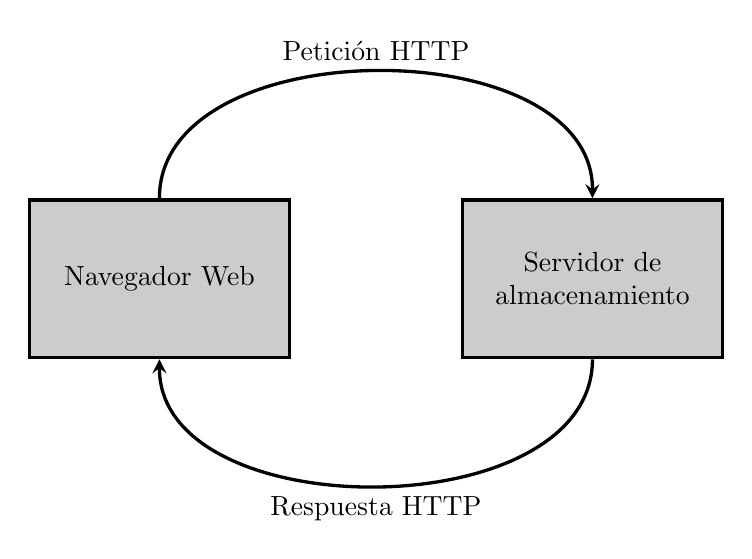
\begin{tikzpicture}
	\tikzstyle{box} = [draw,inner sep=7,minimum size=57,line 
	width=1, very thick, draw=black, fill=black!20, text width=80, text centered]
	\tikzstyle{invisible} = [outer sep=0,inner sep=0,minimum size=0]
	\tikzstyle{stealth} = [-stealth]
	\node [box] (v1) at (0,0) {Navegador Web};
	\node [box] (v2) at (5.5,0) {Servidor de almacenamiento};
	
\draw [stealth, in=90, out=90, very thick] (v1) edge node [anchor=south] {Petición HTTP}(v2);
\draw [stealth, in=270, out=270, very thick] (v2) edge node [anchor=north] {Respuesta HTTP} (v1);
\end{tikzpicture}